\chapter{Implementation Details}
\label{chap:Implementation Details}
\ffigure{img/implementation.png}{Spatial joins using a simple grid structure. A simple spatial join algorithm that puts elements into buckets based on their position in a grid. By putting data pointers directly in the buckets instead of referring to a linked list, a layer of indirection is removed, and 3-fold improvement is observed. Courtesy of \cite{Sidlauskas2014-ef}.}{fig:implementation}

As we move up the memory hierarchy, careful implementation becomes more important. Recent work by Sidlauskas \ea~claims there is a challenge in concluding about data structures and algorithms only for in-memory databases, as the implementation also plays a significant role in performance \cite{Sidlauskas2014-ef}. For instance, if an extra layer of indirection is removed for an algorithm, as seen in Figure \ref{fig:implementation}, we observe a 3-fold performance improvement. 

We have decided to dedicate an entire chapter to \textit{implementation details}, and explain how performance can be improved by reducing the number of branches, avoiding layers of indirection, and utilizing CPU caches.

In this chapter, we will first cover basic theory about modern CPUs. We will then discuss techniques employed by systems studied in this research.

\newpage

\section{Background Information on Modern CPUs and Compilers}
\label{sec:Background Information on Modern CPUs and Compilers}
Modern processors are capable of performing an enormous amount of calculations per second, but that depends on the amount of available and independent work. The instructions-per-second (IPC) difference between minimal and maximal CPU utilization can easily be an order of magnitude \cite{Boncz2005-wj}. Hence, database software must be implemented such that it fully exploits the processing power made available by the CPU.

\subsection{Pipelining, Superscalar Processing, and Independent Instructions}
\label{sub:Pipelining, Superscalar Processing, and Independent Instructions}
\afigure{img/superscalar.png}{A simple superscalar pipeline. Multiple execution units allows for processing multiple instructions in parallel. Courtesy of \cite{Wikipedia_contributors2015-kp}.}{fig:superscalar}{0.6} 

Modern processors improve clock rate and IPC by using a technique known as \textit{pipelining} \cite{Boncz2005-wj}. By dividing an instruction execution into multiple steps, there is less work per stage, and the CPU frequency can be increased. Figure \ref{fig:superscalar} depicts an example pipeline with five stages. However, pipelining also introduce two dangers; \textit{instruction dependencies} and \textit{branch misprediction}.

In a pipeline, \textit{dependencies between instructions} impose a problem. If an instruction is dependent on another, it must wait for the other instruction to complete before it enters the pipeline. Dependent instructions can severely hurt performance, especially if the pipeline is long.

Conditional branches are also affected by dependencies between instructions. When executing a conditional branch instruction, the decision whether to take a branch is usually dependent on the result of a preceding instruction \cite{Boncz2005-wj}. To avoid stalling the pipeline when waiting for the expression to evaluate, modern CPUs use a technique known as branch prediction where the processor immaturely starts executing the branch that is most likely to be taken. The performance penalty occurs if a branch is \textit{mispredicted}, where the instructions in the pipeline must be invalidated (pipeline flushing).

We briefly discussed superscalar processors in Section \ref{sec:Instruction Level Parallelism}. A superscalar processor has multiple execution units to enable IPC $> 1$, and to fully utilize the processor; independent work is required.

\begin{figure}
  \centering
  \begin{subfigure}{0.45\textwidth}
    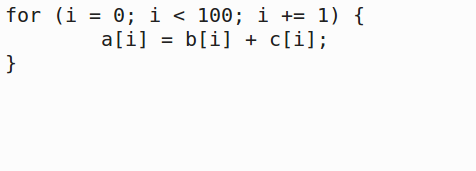
\includegraphics[width=\textwidth]{img/loop-unrolling-1.png}
    \caption{Original loop}
    \label{fig:loop-unrolling-1} 
  \end{subfigure}
  \begin{subfigure}{0.45\textwidth}
    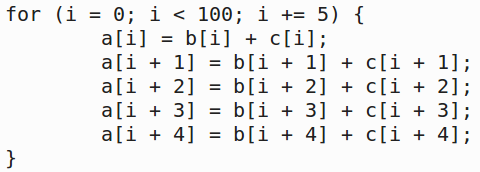
\includegraphics[width=\textwidth]{img/loop-unrolling-2.png}
    \caption{Unrolled loop}
    \label{fig:loop-unrolling-2} 
  \end{subfigure}
  \caption{By unrolling loops, instructions are made independent and the number of branches is reduced.}
  \label{fig:loop-unrolling} 
\end{figure}
Hence, to reach maximum performance on a pipelined, superscalar processor, we must find independent work. Since most programming languages do not let the programmer specify which instructions are independent of each other, compiler optimizations play a critical role in CPU utilization \cite{Boncz2005-wj}. The most widely used technique used by the compilers to address this challenge is through \textit{loop unrolling}, which is used to reduce the number of branches and increase independence between instructions \cite{Wikipedia_contributors2015-zc}. As seen in Figure \ref{fig:loop-unrolling}, loop unrolling reduces the number of iterations in a loop (reduction of branches) and replaces it with multiple instances of the same instruction. If the instructions are independent, they can be processed in parallel.

\subsection{CPU Caches}
\label{sub:CPU Caches}
Since transfering data from main memory to CPU can take around $~200$ cycles, modern CPUs utilize multiple layers of on- and off-chip caches to reduce this latency. Efficient usage of caches is paramount for CPU throughput, since roughly 30\% of all instructions in a program are memory loads or stores \cite{Boncz2005-wj}. We know that IPC for DBMSes is strongly impaired by cache misses, and cache utilization is an important topic for in-memory databases \cite{Exasol2014-xh}.

The best way to tackle this challenge is to design algorithms and data structures that are \textit{cache aware} \cite{Farber2012-vh}. Designing such programs is out of the scope of this report, but it briefly boils down to two things:
\begin{itemize}
  \item \textit{Coordinate temporal and spatial locality}. Data processed together should be stored at consecutive memory addresses. Code locality is also important \cite{Neumann2011-uq}.
  \item \textit{Avoid false sharing of cache lines}. Multiple cores in a processor should not write to data belonging to the same cache entry at the same time to avoid unecessary invalidations.
\end{itemize}
\textit{Compression}, which is described in Chapter \ref{chap:Data Compression}, and \textit{vectorized execution}, which we discuss in Section \ref{sec:Loop Pipelining and Vectorized Execution}, are two techniques used to improve cache performance \cite{Larson2013-mc, Lemke2010-is}.

\textit{Prefetching} is another method used to increase cache utilization. Prefetching proactively loads data into caches such that the data is available when an instruction needs it.

\subsection{Call Stack and Subroutine Invocations}
\label{sub:Call Stack and Subroutine Invocations}
\afigure{img/call-stack.png}{A call stack for a program in execution. Each stack frame contains input parameters, function return address, and local variables for a subroutine invocation. Courtesy of \cite{Wikipedia_contributors2015-od}.}{fig:call-stack}{0.5}

A \textit{call stack} is commonly used in a computer program to store information and state about active subroutines \cite{Wikipedia_contributors2015-od}. Each time a subroutine is called, a \textit{stack frame} is added to the call stack that stores the input arguments, return address, and variables local to the subroutine. See Figure \ref{fig:call-stack}. The call stack can be implemented in both hardware and software, and the implementation varies between different systems. This stack-based technique implies that calling a subroutine comes at a cost; registers must be stored on the stack, and a new stack frame must be added.

Trading off time with space is usually done to address the above challenge; adding more code to improve program efficiency. \textit{Function inlining} is a technique used by compilers where the subroutine code is copied into the callee's body. This way, no new stack frame is created for the subroutine, avoiding the overhead associated with a function invocation.

\textit{Macro expansion} is another form of code generation. Macros are normally specified by the application programmer, and can be used for programmer-controlled inlining of functions or constant values. Macros can also be used to generate multiple versions of function or class definitions (templating), a technique commonly used to support different data types.

\section{Branch Avoidance}
\label{sec:Branch Avoidance}
\ffigure{img/branch-selectivity.png}{Predicate evaluation performance for queries with different query selectivities. A \textit{branch version} and a \textit{predicated version} is tested. For the AthlonMP processor, the branch version are 2-3 times slower on queries with 40\%-60\% selectivity, while the Itanium2 processor has constant processing time. The predicated version offers constant processing time for both processors. Courtesy of \cite{Boncz2005-wj}.}{fig:branch-selectivity}

We saw in the previous section that branches should be avoided due to the penalties of branch misprediction. Besides, branch avoidance might also increase instruction independence.

The consequences of inaccurate branch prediction are studied by Neumann \ea~\cite{Neumann2011-uq}. In this research, the performance of queries with various selectivities was tested. As we can see in Figure \ref{fig:branch-selectivity}, queries with 40\%-60\% selectivity executed on an AthlonMP processor are roughly 2-3 times slower than queries with selectivities close to 0\% or 100\%. Hence, selectivity can severely affect the query performance. The Itanium2 processor does not have the same characteristic, as the Itanium architecture allows for both \textit{not taken} and \textit{taken} branches to be executed simultaneously.

Neumann \ea~also developed a branchless version (predicated version) to evaluate predicates in the queries. The branchless variant is denoted as \texttt{predicated version} in Figure \ref{fig:branch-selectivity}. For both AthlonMP and Itanium2 processors, this implementation offers constant performance for all selectivities, but is, in general, more expensive.

Branch avoidance is also important in other parts of the system, like decompressing. Zukowski \ea~present a decompression algorithm that is free for \textit{if-then-else} statements \cite{Zukowski2006-oz}. By running the algorithm in two tight loops instead of one, branch misprediction is reduced, and the loops can be pipelined by a compiler.

Branches can also be avoided by compiling queries to machine code \cite{Lamb2012-kg}. We study this technique in greater detail in Section \ref{sub:Compiling Queries to Machine Code}.

\subsection{Short-circuiting}
\label{sub:Short-circuiting}
\begin{figure}
  \centering
  \begin{subfigure}{0.45\textwidth}
    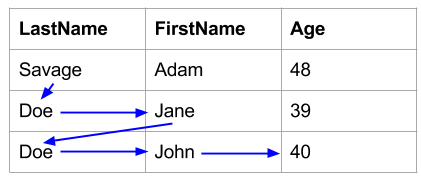
\includegraphics[width=\textwidth]{img/short-circuiting-1.png}
    \caption{Short-circuiting}
    \label{fig:short-circuiting-1} 
  \end{subfigure}
  \begin{subfigure}{0.45\textwidth}
    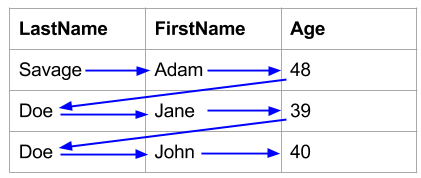
\includegraphics[width=\textwidth]{img/short-circuiting-2.png}
    \caption{No short-circuiting}
    \label{fig:short-circuiting-2} 
  \end{subfigure}
  \caption{Predicate evaluation for query \texttt{WHERE LastName='Doe' AND FirstName='John' AND Age>21}. (a) skips evaluating rest of the predicates if one predicate is false, while (b) evaluates all predicates regardless of previous results.}
  \label{fig:short-circuiting} 
\end{figure}
\textit{Short circuiting} is referred to a special case of Boolean operator evaluation in which the next argument is not evaluated if the current argument is sufficient to determine the value of the expression \cite{Wikipedia_contributors2015-rk}. Figure \ref{fig:short-circuiting} illustrates the difference between short-circuit and non-short-circuit predicate evaluation. In short-circuiting, the scan proceeds to the next tuple as soon as one predicate is false, as opposed to the verision without short-circuiting that evaluates all predicates regardless of previous results.

Since short-circuit boolean operators are control structures and not simple arithmetic operators, there is a chance of branch misprediction. That is why \blink~\cite{Raman2008-gi, Johnson2008-cp} does not short circuit between tuples. If a block is selected for scanning, all fields in a record are checked. According to Raman \ea, short-circuiting only improves performance on low selectivity queries \cite{Raman2008-gi}.


\section{Loop Pipelining and Vectorized Execution}
\label{sec:Loop Pipelining and Vectorized Execution}
The absence of loop pipelining can have dramatic effects on query performance \cite{Boncz2005-wj}. Boncz \ea~show that \mysql~uses 49 cycles per tuple due to the absence of loop pipelining. In \mysql, there are 1-2 funcion calls to extract the needed data from a tuple for each iteration \cite{Abadi2008-dd}. Evaluating a predicate is usually a small operation compared to the overhead associated with calling subroutines, which means most of the 49 instructions are spent managing the call stack.

In order to ensure proper loop pipeline behavior, compilers must know that pointers do not overlap, such that loop unrolling can be used \cite{Boncz2005-wj}. In \monetx, this is made explicit by passing CPU primitives that expose to the compiler that processing a tuple is independent from the others.

To avoid unecessary subroutine invocation overhead and help the compiler identify which instructions are independent, \textit{vectorized execution} is normally used.

\subsection{Vectorized Execution}
\label{sub:Vectorized Execution}
Vectorized execution, or block iteration, is the technique where multiple rows are processed at the same time to avoid the overhead associated with tuple-at-a-time processing \cite{Abadi2008-dd}. Vectorized execution enables loop unrolling, memory prefetching, and minimizing of cache misses \cite{Larson2013-mc}. Research executed by Abadi \ea~shows that vectorized execution in columns stores improves performance by 50\% on average.

% explain who uses it
Several systems studied in this report use vectorized execution. \ibm~and \mssql~work on batches of thousands of row at a time \cite{Larson2013-mc, Raman2013-em}. \monetdb~and \monetx~use vectors instead of single values as their main structure for storing data \cite{Boncz2002-yj, Boncz2005-wj}. Vectorized execution is also used by \cstore~and \blink \cite{Johnson2008-cp, Stonebraker2005-qz}.

% Explain how it works.
\afigure{img/vectorized-execution.png}{\mssql~operates on row batches. Each row batch has a vector for each column and a bit vector indicating qualifying rows. Courtesy of \cite{Larson2013-mc}.}{fig:vectorized-execution}{0.4}
In vectorized execution, blocks of values from the same column are sent to an operator for evaluation \cite{Zukowski2006-oz}. \mssql~works on batches of columns at the same time, which is seen in Figure \ref{fig:vectorized-execution}. Here, all columns are evaluated using tight loops. A bit vector indicating qualifying rows is where the results are stored. Regarding vector size, vectors should not be too small due to increased overhead and less parallelism, nor too big, as it should fit in CPU cache \cite{Boncz2005-wj}.

Although vectorized execution for column stores normally outperform tuple-at-a-time query processing, there are some disadvantages using this model. Neumann \ea~claim that vectorized execution eliminates a major strength of the iterator model, namely \textit{pipelining} \cite{Neumann2011-uq}. In this context, pipelining means the ability for an operator to pass tuples to its parent operator without copying the value. When vectorized execution is used, intermediate results have to be stored somewhere (materialized), which consumes memory bandwidth.

\section{Code Generation}
\label{sec:Code Generation}
In Section \ref{sub:Call Stack and Subroutine Invocations}, we briefly discussed how code generation can be used to avoid overhead related to function invocations. In this section, we study two techniques employed by systems studied in this research.


\subsection{Compiling Queries to Machine Code}
\label{sub:Compiling Queries to Machine Code}
Compiling queries to machine native code can be used to increase the performance of expression evaluation, to avoid branches, and reduce the number of function calls \cite{Lamb2012-kg, Neumann2011-uq}. It is particularly effective for ad-hoc queries \cite{Psaroudakis2014}. Systems compiling queries into machine code include \blink~\cite{Barber2012-xt}, \ibm~\cite{Raman2013-em}, \vertica~\cite{Lamb2012-kg}, \hyper~\cite{Psaroudakis2014-ma}, and \mssql~\cite{Delaney2014-ip}. This technique is also employed by \qlikview, and has been claimed that compilated code vs interpreted code gives up to 5X performance for this product \cite{noauthor_undated-js}.

Before compiling queries from value to code space, \blink~looks up keys in the dictionary which are used to generate code \cite{Barber2012-xt}. Hence, scans can be performed directly on the compressed data without looking up values in the dictionary. Since different partitions have different dictionaries, a query must be compiled per partition. 

Data structures and functions for data access can also be compiled to machine code. \mssql~compiles memory-optimized tables and stored procedures that are used to access them \cite{Delaney2014-ip}. This allows for more efficient query execution than the traditional interpreted SQL. Using the Visual C compiler, a dynamic linked library (DLL) per table is created and linked into the \mssql~process.

\begin{figure}
  \centering
  \begin{subfigure}{0.45\textwidth}
    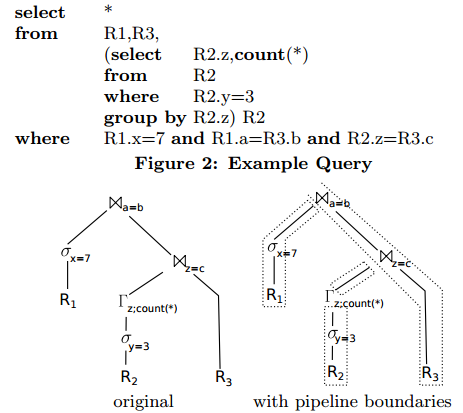
\includegraphics[width=\textwidth]{img/pipeline-boundary-1.png}
    \caption{...}
    \label{fig:pipeline-boundary-1} 
  \end{subfigure}
  \begin{subfigure}{0.45\textwidth}
    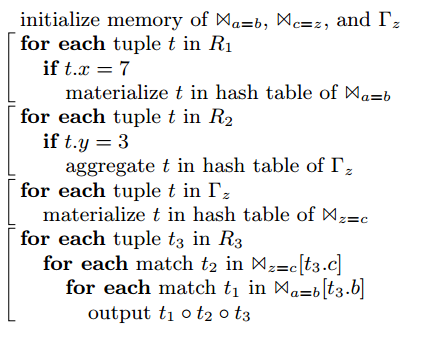
\includegraphics[width=\textwidth]{img/pipeline-boundary-2.png}
    \caption{...}
    \label{fig:pipeline-boundary-2} 
  \end{subfigure}
  \caption{Pipeline boundaries. Courtesy of \cite{Neumann2011-uq}.}
  \label{fig:pipeline-boundary} 
\end{figure}

Neumann~\ea have identified the need for machine code compilation of queries \cite{Neumann2011-uq}. Even though vectorized execution has come a long way to utilize modern CPUs, such plans are frequently outperformed by handwritten execution plans. Hand-written queries are data-centric and not operator-centric, in addition to avoiding uncessecary materialization steps.

To counter the challenges with vectorized execution, queries was compiled into native machine code using the LLVM compiler framework.

As seen in Figure \ref{fig:pipeline-boundary}, by turning the query from operator centric to data centric, uneccesary data materialization can be avoided by executing several operators on the data at the same time. This way, the data is left in the CPU registers and only utilize memory to retrieve new tuples or to materialize the results. Besides, the complied code has tight loops with good code locality that works on large amounts of data.


Vectorized execution, as described in Section \ref{sub:Vectorized Execution}, improves performance on modern CPUs, but such techniques are frequently out-performed by hand-written execution plans \cite{Neumann2011-uq}. The work by Neumann \ea~\cite{Neumann2011-uq} explains how queries are compiled into native machine code using the LLVM compiller framework. Doing this, the processing of queries are data centric and not operator centric. Classical query processing always wipes the CPU registers, but in their solution they push tuple values until a pipeline is broken. They tried using the C++ compiler, but it turned out too slow. Therefore, the major application was developed in C++.

\subsection{Macro Expansions}
\label{sub:Macro Expansions}
\afigure{img/macro-expansion.png}{Macro expansions in \monetdb. For different algorithms and data types, the \texttt{select} operator has a total of 173 implementations. Courtesy of \cite{Boncz2002-yj}.}{fig:macro-expansion}{0.6}
\monetdb~uses macro expansion to reduce layers of indirection optimize query execution performance \cite{Boncz2002-yj}. Since operators normally are type-generic, \monetdb~has for each algorithm multiple implementation routines that are specific to a certain type. The implementations are generated automaticly using macros, hence they are called \textit{macro expansions}. Figure \ref{fig:macro-expansion} shows how the select operator is expanded into 173 implementations, depending on which alorithm and data types are queried.



\section{Cache Awareness and Prefetching}
\label{sec:Cache Awareness and Prefetching}
We saw in Section \ref{sub:CPU Caches} that efficient utilization of caches is important for database performance. In terms of database algorithm, several cache aware variants have been proposed. \monetdb~\cite{Boncz2002-yj} introduce a clever clustering algorithm called \term{radix cluster}, where cache utilization is maximized by performing muliple passes over the data. \oracle~\cite{Lahiri2015-mz} uses an algorithm known as \term{Vector Group By}, which is a compact multidimensional array for storing aggregate results.

Prefetching is the act of getting data up the storage hierarchy before the data is actually needed. Prefetching is made available to the processors if vectorized execution is used. Explicit prefetching is used by several systems, like \ibm~\cite{Raman2013-em}, \monetx~\cite{Boncz2005-wj}. \exasol~uses special CPU instructions to prefetch certain memory locations to improve data locality \cite{Exasol2014-xh}.
\todo{Consider skipping the entire section}



\section{Chapter Conclusion}
\label{sec:Chapter Conclusion}

